\documentclass{beamer}
\usepackage[utf8]{inputenc}

\usepackage{xeCJK}

\usetheme{Madrid}
\usecolortheme{default}

\title{2022年秋季招新线上培训}
\subtitle{性能优化的基础知识与基本方法简述}
\author{七边形超算队}
\institute{华中科技大学}
\date{2022年11月21日}
\logo{
\includegraphics[height=1cm]{heptagon.jpg}}

\AtBeginSection[]
{
  \begin{frame}
    \frametitle{目录}
    \tableofcontents[currentsection]
  \end{frame}
}

\begin{document}

%The next statement creates the title page.
\frame{\titlepage}

%---------------------------------------------------------
%This block of code is for the table of contents after
%the title page
\begin{frame}
\frametitle{目录}
\tableofcontents
\end{frame}
%---------------------------------------------------------


\section{性能优化的量度}

%---------------------------------------------------------
%Changing visivility of the text
\begin{frame}
\frametitle{加速比和效率}

\begin{itemize}
    \item<1-> HPC比赛的主要内容是对程序进行性能优化,而评估优化效果的一个直观方法是:插入计时代码,然后计算加速比。
    \item<2-> 假设一个程序原本的运行时间为$T_0$,优化后的运行时间为$T$,我们定义加速比$S$为两者的比值,即$S=T_0/T$。例如:若一个程序原本运行时间为$10s$,优化后的运行时间为$0.1s$,则该程序取得了$100$倍的优化比。
    \item<3-> 对于并行优化来说,假设有$p$个核同时执行程序,则程序的理想加速比也为$p$。但很多时候,由于串行部分的存在,以及并行部分在通信与同步上的花费等,程序难以被完全并行化,因此难以达到理想加速比。我们定义一个指标:效率$E=S/p$,用来量化地描述所有参与计算的核心是否得到了充分的利用。
    \item<4-> 一般来说,拥有更加出色的效率$E$的程序,其并行程度更高,并且具有更好的可扩展性。
\end{itemize}

\end{frame}

\begin{frame}
\frametitle{阿姆达尔定律}
\begin{itemize}
    \item<1-> 一个程序的加速比除前述的定义式外,也可以被表示为$\frac{W_s+W_p}{W_s+W_p/p}$,式中$W_s$与$W_p$分别表示问题规模的串行分量(问题中不能并行化的那一部分)和并行分量,$p$表示处理器数量。
    \item<2-> 注意到当$p→+∞$时,上式的极限是$\frac{W_s+W_p}{W_s}$。这意味着无论如何增大参与计算的处理器核心数目,加速比都是无法高于这个值的。也就是说,未能被并行化的部分会成为这个优化过程的一个瓶颈。
\end{itemize}
\end{frame}

\section{串行优化简述}

%---------------------------------------------------------
%Highlighting text
\begin{frame}
\frametitle{概述}

\begin{itemize}
    \item<1-> 串行优化的主要目标,是通过直接降低计算量来达到加速的目的。
    \item<2-> 首先,直接采用更优复杂度的算法当然是效果显著的优化方法。
    \item<3-> 除此以外,还有一些我们平时比较容易忽略的编程细节可能会对性能造成一定影响。以下挑选几个典型的例子进行说明。
\end{itemize}

\end{frame}

\begin{frame}
\frametitle{消除重复计算}
一模一样的计算被反复进行,是较为常见的一种情况,会带来不可小觑的性能问题。下图是一段把字符串中的大写字母转换为对应小写字母的程序。

注意:C语言库中的strlen()是一个O(n)复杂度的调用。

\centering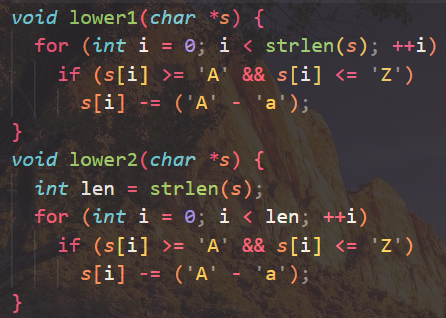
\includegraphics[height=4cm]{reducecalc.png}\pause
\centering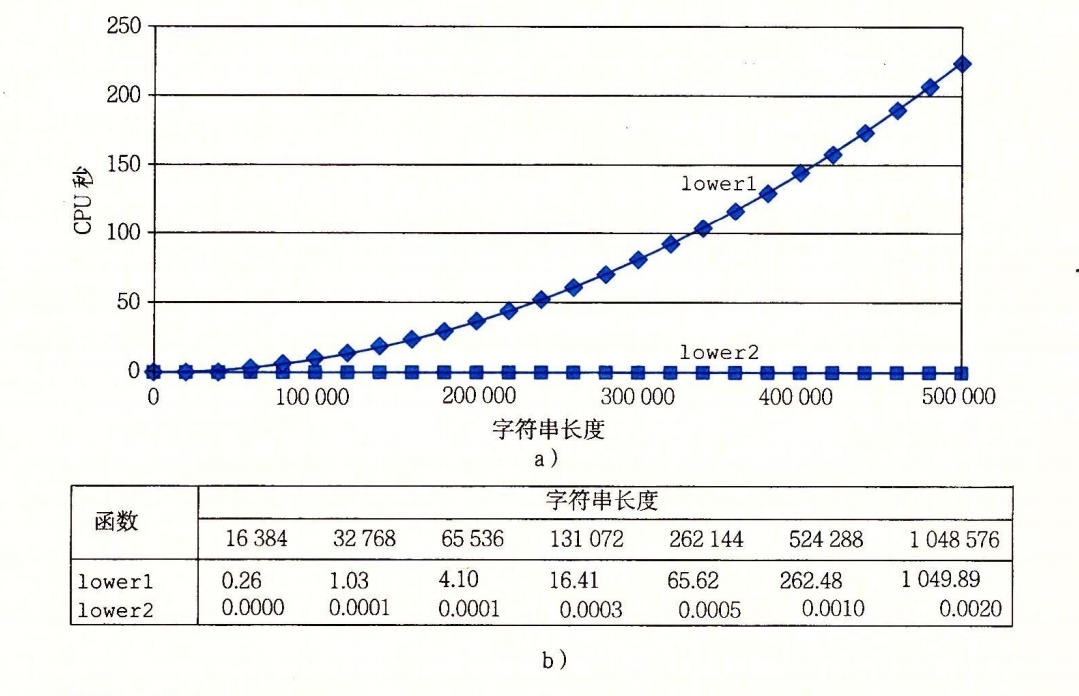
\includegraphics[height=4cm]{benchmark0.jpg}
\end{frame}

\begin{frame}
\frametitle{循环展开}

\begin{itemize}
    \item<1-> 循环展开是一种程序变换,通过增加每次迭代计算的元素数量,减少循环的迭代次数。
    
    \centering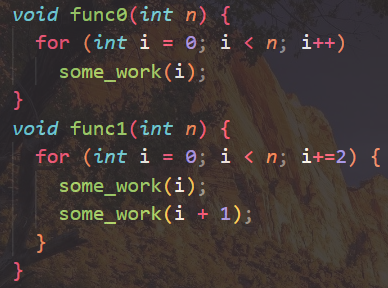
\includegraphics[height=4cm]{for.png}\pause

    \item<2-> 这种方法减少了循环索引计算、条件分支等不必要的冗余开销,在单次迭代计算量较低的时候会产生更好的效果。
\end{itemize}


\end{frame}

\section{并行优化简述}

\begin{frame}
\frametitle{概述}
\begin{itemize}
    \item<1-> 并行优化的主要目标,是将庞大的计算量拆分之后进行并行处理,从而在总计算量不变的同时达到显著的加速效果。
    \item<2-> 有多种实现路径,下面主要介绍数据级并行和线程级并行的思想。
\end{itemize}
\end{frame}

\begin{frame}
\frametitle{数据级并行}
\begin{itemize}
    \item<1-> SIMD全称Single Instruction Multiple Data,单指令多数据流。这种方法依靠处理器中专门的处理单元,通过复制多个操作数、并把它们打包在向量寄存器里执行批量计算的一组指令集来实现。可以在处理器厂商提供的文档中查阅其SIMD指令集的使用指引。
\end{itemize}
\centering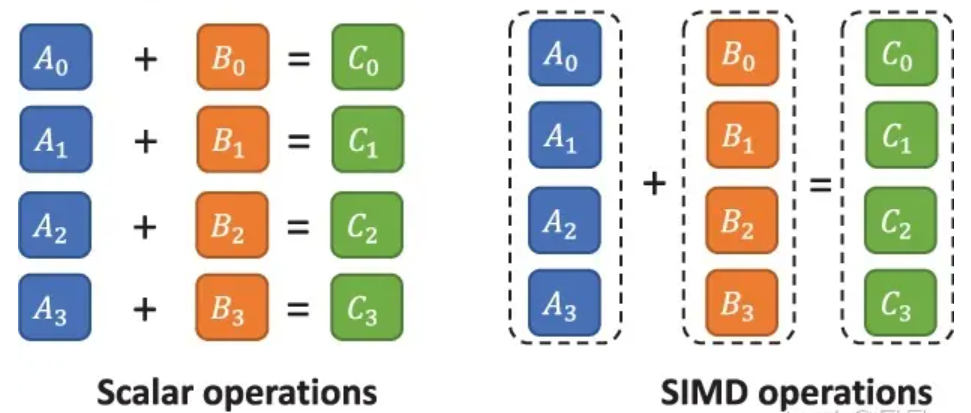
\includegraphics[height=3cm]{simd.png}
\end{frame}

\begin{frame}
\frametitle{数据级并行}

\begin{block}{代码示例:使用 Intel AVX-512 指令集进行向量加法计算}
\centering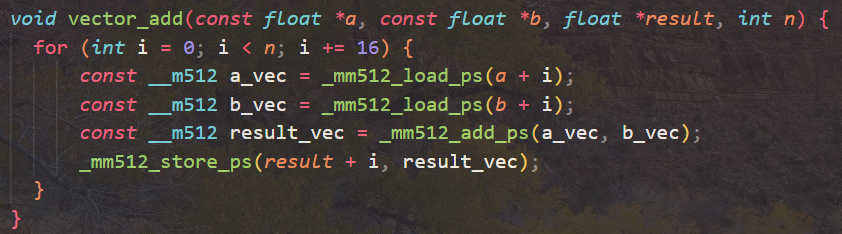
\includegraphics[height=3cm]{simd_code.png}
\end{block}
\end{frame}

\begin{frame}
\frametitle{线程级并行}
\begin{itemize}
    \item<1-> 线程(thread)是操作系统能够进行运算调度的最小单位。在多核处理器早已普及的当下,几乎所有的计算机都支持多个线程同时执行。
    \item<2-> 然而,我们编写的程序,默认是只会在一个线程中执行的,若要使用多个线程来执行我们指定的任务,需要我们在编程时进行一些额外的工作来进行线程调度。某种意义上说,使程序具备并行性是程序编写者的任务,而非编译器的。
    \item<3-> 几乎所有的高级语言都对线程级并行提供支持,下面以C++语言为例介绍两种常用方法:C++ thread 库和 OpenMP 框架。
\end{itemize}
\end{frame}

\begin{frame}
\frametitle{std::thread}
C++的 <thread> 头文件中有 std::thread 类,提供线程的创建、回收等能力。

\centering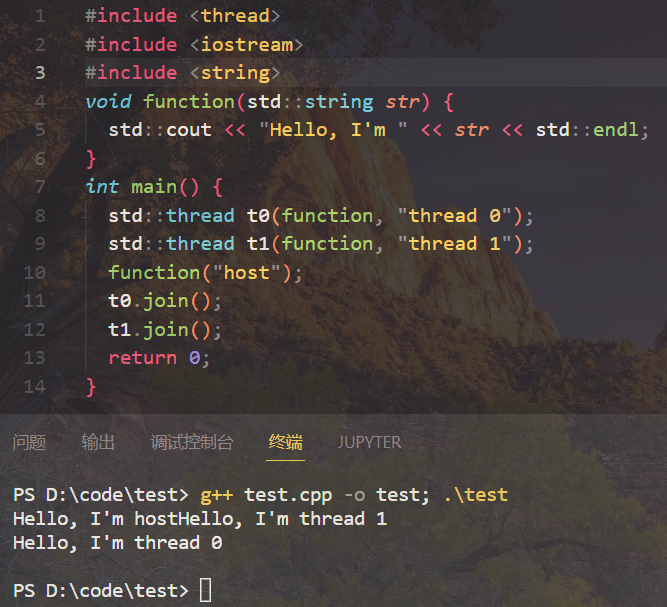
\includegraphics[height=6cm]{thread.png}
\end{frame}

\begin{frame}
\frametitle{OpenMP}
OpenMP框架提供更加便捷的多线程编程方式,通过一条#pragma预处理指令将后续紧邻的一行或一段程序声明为并行执行,并由编译器进行处理。可以通过在预处理指令后追加参数来调整任务在线程间分配的细节。

\centering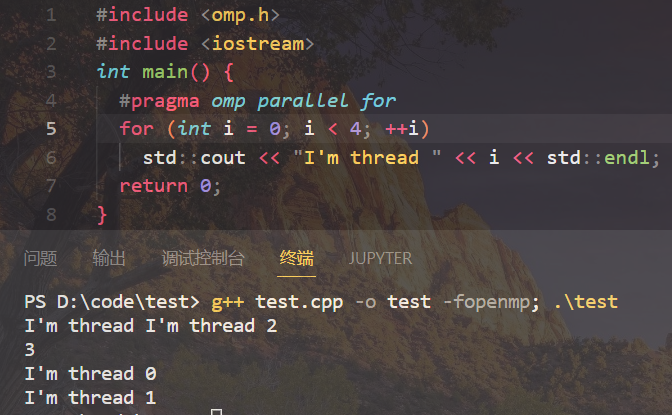
\includegraphics[height=5cm]{openmp.png}
\end{frame}

\begin{frame}
\frametitle{OpenMP}

\begin{block}{代码示例:使用 OpenMP 进行并行加法计算}
\centering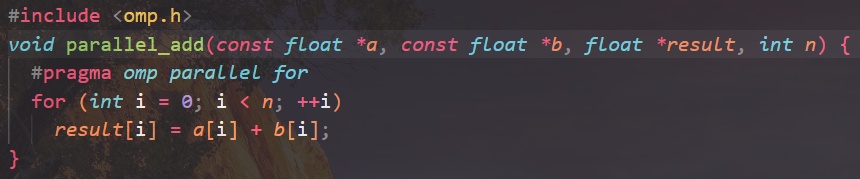
\includegraphics[height=2.5cm]{parallel_add.png}
\end{block}
\end{frame}

\begin{frame}
\frametitle{一些拓展}
\begin{itemize}
    \item<1-> 以下内容相比之下属于高级主题,有兴趣的同学可以自行探索了解。
    \item<2-> 从单机计算拓展到集群计算(MPI等)
    \item<3-> 操控并行计算能力更强大的GPU等设备进行计算(CUDA等)
\end{itemize}
\end{frame}

\section{访存优化简述}

%---------------------------------------------------------
%Changing visivility of the text
\begin{frame}
\frametitle{概述}
\begin{itemize}
    \item<1-> 很多时候,数据的读写会占用较多的时间,有时甚至比计算部分更加拖累程序的整体性能。因此,除前述的计算层面的优化外,访存的优化往往也是重要的。
    \item<2-> 在此着重分享一个话题:Cache的特性,及其带来的访存局部性问题。
\end{itemize}

\end{frame}

\begin{frame}
\frametitle{计算机存储体系}
\begin{itemize}
    \item 计算机的存储结构实际上是一个层次化的结构。最顶层的寄存器速度最快,但单位容量的成本十分高昂;靠近底层的硬盘等设备的性能相对较差,但成本低廉,可以用较低成本获得较大容量。
    \item 为了尽可能获得和底层存储器相近的低廉成本的同时,又尽可能接近顶层存储器的优秀性能,所以层次结构应运而生。在这一层次结构中,层次更低的存储器的性能更低但空间更大,并且每一层存储器都作为下一层存储器的缓存。缓存常用的一种策略是LRU策略。
\end{itemize}
\centering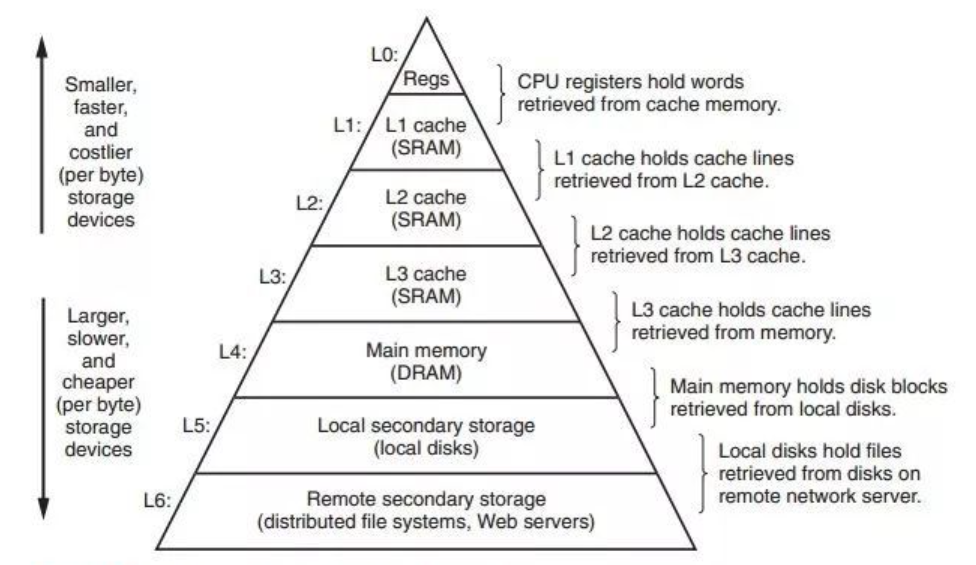
\includegraphics[height=4cm]{memory.png}
\end{frame}

\begin{frame}
\frametitle{局部性问题的产生}
\begin{itemize}
    \item<1-> 如此,便产生了时间局部性和空间局部性问题。
    \item<2-> 由于每一层存储器都会缓存最近刚被访问的数据,所以如果我们在短时间内多次访问同一个地址,那么该地址对应的数据将很有可能仍在高层存储器中留存,可以直接取用,获得出色的访存性能。如果反之,我们对某个位置的多次访问在时间上是相隔久远的,那将难免每次都需要访问低层存储器,从而造成严重的性能损失。这就是时间局部性问题。
    \item<3-> 由于每层存储器向下一层存储器读取数据时,会一次性读取其后的连续一段数据,所以如果我们连续访问位置上相邻的数据,往往将有大多数请求可以由高层存储器直接响应。如果反之,我们在访存时不遵循连续访存的原则,而是跳跃访存,那也将难免造成性能损失。这就是空间局部性问题。
\end{itemize}
\end{frame}

\section{答疑}

\begin{frame}
\frametitle{答疑}
Waiting for questions...
\end{frame}

\end{document}